\documentclass{mmposter}

\colorlet{CEmphasis1}{clustercassis}
\colorlet{CEmphasis2}{clusterblue}

\usepackage{lipsum}
\usepackage{blindtext}
\usepackage{tikz}
\usepackage{amsmath}
\usepackage{derivative}
\usepackage{hyperref}
\hypersetup{
	colorlinks,
	citecolor=black,
	urlcolor=CEmphasis1,
}
\usepackage{minted}

\title{Improving Interoperability\\in Scientific Computing\\via MaRDI Open Interfaces}
\authors{Contributors:
	Dmitry I.\ Kabanov, Stephan Rave, Mario Ohlberger
}
\renewcommand{\refname}{References}

\newcommand{\OIF}{\textsc{MaRDI Open Interfaces}\xspace}

\newcounter{hilfszaehler}

\graphicspath{{./assets/}}

\begin{document}
\bibliographystyle{plain}

\maketitle

\section*{Summary}
Computational scientists often face two obstacles while conducting
numerical experiments.
First, there are several popular languages used by numerical
software packages as well as different preferences for a ``driving''
language, in which an experiment's logic is formulated.
Connecting different languages and packages directly requires
developing bindings to for these packages, which can amount
to a significant work.
Second, the programming interfaces between even packages
that solve the same numerical problem, have different interfaces.
Therefore, it requires a significant effort from a computational
scientist, if there is a need to switch from one numerical package
to another, in the flow of the computational project.

The goal of \OIF{} is to improve interoperability in Scientific
Computing by alleviating these obstacles.

\begin{objectives}
  \item Develop library that passes data between languages automatically
  \item Develop Open Interfaces for typical numerical problems,
  such as optimization or integration of differential equations
  \item Spread information about Open Interfaces to encourage
  scientific-computing community to program against these interfaces.
\end{objectives}

\section*{Software Architecture and Data Flow}
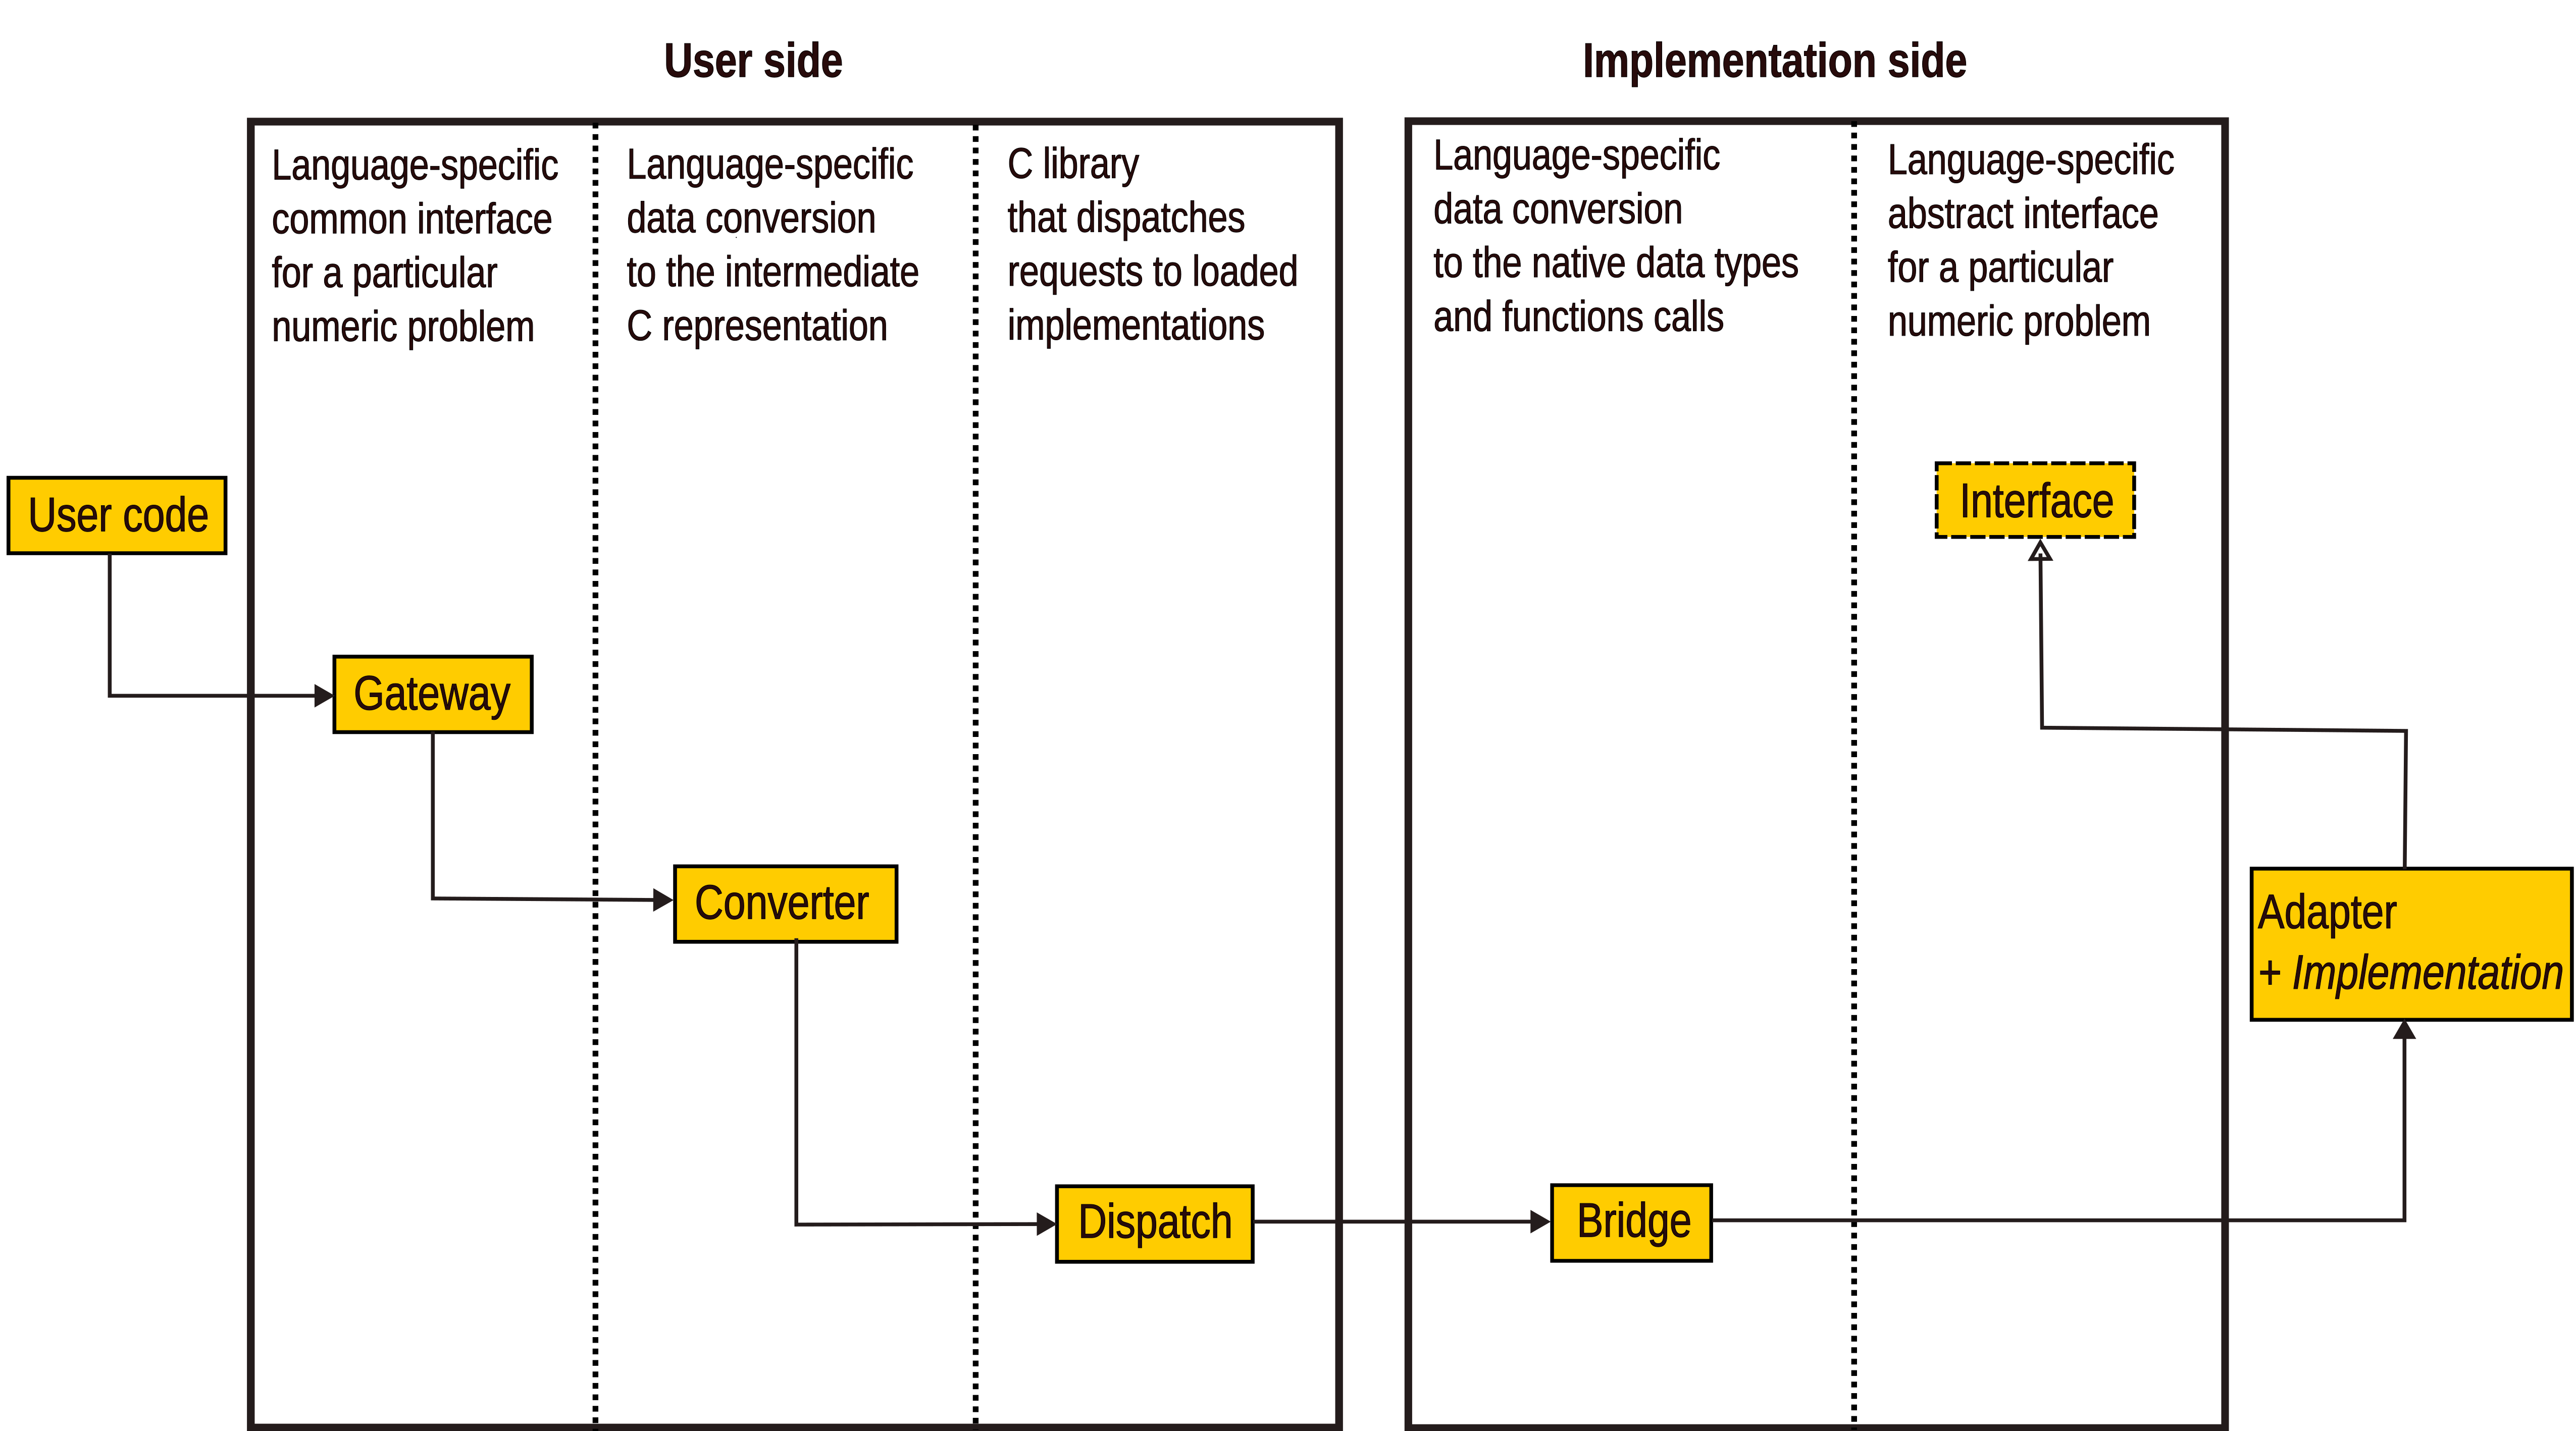
\includegraphics[width=\columnwidth]{arch.png}

\textbf{User} requests an implementation of an Open Interface
and interacts with the implementation only via a \textbf{Gateway},
so that the discrepancies between different implementations in terms
of functions signatures and order of invocation become transparent
to the \textbf{User}.

The function arguments are converted from the user's language
to a C intermediate representation inside a \textbf{Converter}
that passes them further.
The \textbf{Dispatch} is responsible for loading an implementation
and its corresponding runtime (\textbf{Bridge}).
The \textbf{Bridge} converts data from the intermediate representation
to the native data types of the implementation and invokes
the requested function, which also occurs via \textbf{Interface},
that is, the implementation is invoked via an adapter.

\newpage

\section*{Example usage}
Inviscid Burgers' equation:
\begin{align*}
  &\pdv{u}{t} + \pdv{\left( u^{2} / 2 \right)}{x} = 0,
  \quad t \in [0, 2], \quad x \in [0, 2] \\
  &u(t, 0) = 0.5 - 0.25 \sin \left( \pi x \right)\\
  &u(t, 0) = u(t, 2)
\end{align*}
\begin{minipage}{\dimexpr0.46\columnwidth - 2\tabcolsep}
  \textbf{Implementations}:
  \begin{itemize}
    \item Sundials CVODE,\\Adams--Moulton method
    \item \texttt{scipy.integrate.ode},\\Dormand--Prince method
    \item \texttt{OrdinaryDiffEq},\\Tsitouras method
  \end{itemize}
\end{minipage}\hfill%
\begin{minipage}{\dimexpr0.54\columnwidth - 2\tabcolsep}
  % \centering
  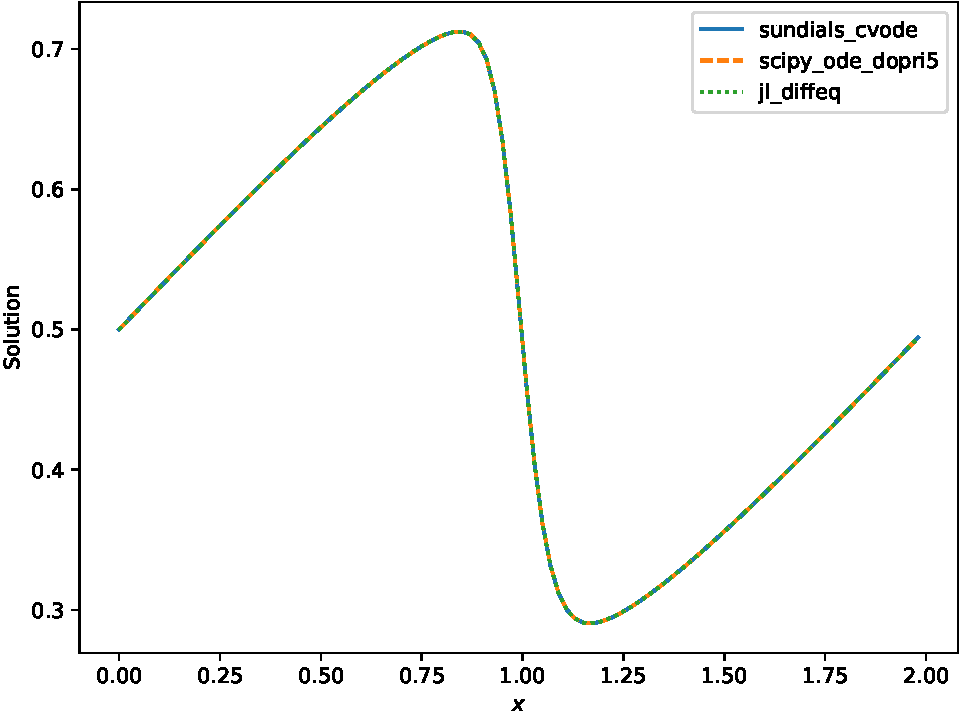
\includegraphics[width=\linewidth]{ivp_c_burgers_eq}
\end{minipage}

\vspace{2em}
\textbf{User code in Python:}
\begin{minted}[autogobble, beameroverlays, escapeinside=||]{Python}
  from oif.interfaces.ivp import IVP
  ...

  # `BurgersEquationProblem` is a utility user class.
  impl = "scipy_ode"
  problem = BurgersEquationProblem(N=1001)
  s = IVP(impl)
  s.set_initial_value(problem.y0, problem.t0)
  s.set_rhs_fn(problem.compute_rhs)

  times = np.linspace(problem.t0, problem.tfinal, num=11)

  soln = [y0]
  for t in times[1:]:
      s.integrate(t)
      soln.append(s.y)
\end{minted}


\section*{Conclusions}
\lipsum[3]

\section*{Connections to other MaRDI subprojects}

\begin{itemize}[align=left]
  \item[\color{CEmphasis1}M2.3:] Benchmarking of MOR software is potentially
    easier using \OIF{}.
  \item[\color{CEmphasis1}M?.?:] Tool that helps with reproducibility
    by ``containerization''.
\end{itemize}

\begin{thebibliography}{1}
  \setlength{\itemsep}{1pt}
  \setlength{\parskip}{1.5pt}

  \scriptsize{

  \bibitem[1]{PyMOR}
  Ren{\'{e}}, M., Rave, S., and Schindler, F.
  \newblock pyMOR -- Generic Algorithms and Interfaces for Model Order Reduction, 2016.
  \newblock doi:10.1137/15m1026614.
  }
\end{thebibliography}

\end{document}
